\documentclass[12pt]{article}

\usepackage{sbc-template}
\usepackage{graphicx,url}
\usepackage{babel}
\usepackage[T1]{fontenc}
\usepackage[utf8]{inputenc}
\usepackage{multicol}
\usepackage{multirow}
\usepackage{amsmath,amssymb,amsfonts}
\usepackage{textcomp}
\usepackage{url}
\usepackage{enumerate}
\usepackage{verbatim}
\usepackage[table,xcdraw]{xcolor}
\usepackage[shortlabels]{enumitem}
\usepackage{fancyhdr}
\usepackage{sbgames}
\usepackage{booktabs}
\usepackage{tikz}
\usetikzlibrary{positioning,arrows.meta,shapes.geometric}

\tolerance=1
\emergencystretch=\maxdimen
\hyphenpenalty=10000
\hbadness=10000

\sloppy


\trilha{Informe a Trilha} %Preencha com: Artes \& Design | Computação | Cultura | Saúde | Indústria | Educação | Tutoriais | MAGICA | WGP-Jogos
\local{Cidade/UF} % Exemplo: Manaus/AM
\ano{20XX} % Exemplo: 2024
\edicao{Edição (Romano)} %Exemplo: XXIII

\title{Avaliação de Sistemas Interativos Baseados em LLM: Um Protocolo Reprodutível para Coerência Narrativa e Consistência de Estado \\
\medskip
\small{
    \textit{Title: Evaluating Interactive LLM-Based Systems: A Reproducible Protocol for Narrative Coherence and State Consistency}
}
}

\author{[OMITIDO PARA REVISÃO ANÔNIMA]}

\address{[OMITIDO PARA REVISÃO ANÔNIMA]
  \email{[OMITIDO PARA REVISÃO ANÔNIMA]}
}

\begin{document}

\maketitle

\thispagestyle{plain}

\begin{abstract}
Evaluating interactive Large Language Model (LLM)-based systems, such as Game Masters in role-playing games (RPGs), remains a challenging problem due to the multi-turn, stateful, and subjective nature of these interactions. This paper presents a reproducible evaluation protocol for interactive LLM-based systems based on LLM-as-a-judge and operating over structured gameplay logs. The protocol is organized around six explicit functional requirements (multi-turn evaluation, state awareness, reproducibility, model-agnostic operation, metric-based assessment, and scalability) and defines a metric-driven pipeline that captures narrative quality, action-to-narration coherence, and state consistency. Unlike prior approaches focused on static or controlled benchmarks, the protocol evaluates full gameplay sessions, enabling analysis of long-term behavior and state evolution, and supports local LLM deployment for reproducibility. The protocol effectively differentiates system performance across four open-weight models (Qwen2.5 family at 0.5B, 1.5B, 7B; Gemma 4 effective 2B) over 10 sessions with 3 human players (30 to 60 rounds each), and identifies five recurring failure modes (internal-variable leakage, history-contamination hallucinations, persona breaks with meta-apologies, system-prompt structure leakage, and explicit admission of technical limitations), all more frequent in models below 7B parameters. The proposed protocol provides a practical and extensible framework for evaluating interactive, stateful LLM-based systems.
\end{abstract}

\keywords{Large Language Models, Game AI, Evaluation Methods, Interactive Systems, Narrative Generation, LLM-as-a-Judge.}

\begin{resumo}
A avaliação de sistemas interativos baseados em Modelos de Linguagem de Grande Escala (LLMs), como Mestres de Jogo em RPGs, é um problema desafiador devido à natureza multi-turno, com estado e subjetiva dessas interações. Este trabalho apresenta um protocolo reprodutível de avaliação para sistemas interativos baseados em LLM, fundamentado em LLM-as-a-judge e operando sobre logs estruturados de \textit{gameplay}. O protocolo é estruturado em torno de seis requisitos funcionais explícitos (avaliação multi-turno, consciência de estado, reprodutibilidade, operação agnóstica de modelo, avaliação baseada em métricas e escalabilidade) e define um \textit{pipeline} orientado a métricas que capta qualidade narrativa, coerência ação\,/\,narração e consistência de estado. Diferente de abordagens centradas em \textit{benchmarks} estáticos, o protocolo avalia sessões completas de jogo, viabilizando análise de comportamento de longo prazo, e suporta execução local para reprodutibilidade. Resultados experimentais com quatro modelos de pesos abertos (Qwen2.5 em 0.5B, 1.5B e 7B; Gemma~4 effective~2B) e 3 jogadores humanos (10 sessões, 30 a 60 rodadas cada) demonstram que o protocolo diferencia consistentemente o desempenho dos sistemas e identifica cinco modos recorrentes de falha (vazamento de variáveis internas, alucinações por contaminação de histórico, quebra de persona com meta-desculpas, exposição da estrutura do prompt de sistema e admissão explícita de limitação técnica), todos mais frequentes em modelos abaixo de 7B parâmetros. O protocolo proposto fornece um arcabouço prático e extensível para avaliação de sistemas interativos baseados em LLM com estado.
\end{resumo}

\palavraschave{Modelos de Linguagem, IA em Jogos, Métodos de Avaliação, Sistemas Interativos, Geração Narrativa, LLM-as-a-Judge.}

% ─────────────────────────────────────────────────────────────────────────────
\section{Introdução}

Jogos de RPG de mesa (\textit{tabletop RPG}) dependem de um Mestre de Jogo (MJ) humano para conduzir a narrativa, arbitrar regras e manter a consistência do mundo. Com o avanço dos Grandes Modelos de Linguagem (LLMs), tornou-se possível automatizar parcialmente essas funções, criando MJs artificiais capazes de gerar narrativas interativas.

No entanto, a \textbf{avaliação} desses sistemas permanece um desafio aberto. A qualidade narrativa, a coerência entre ações e descrições e a consistência de estado ao longo de múltiplas interações são aspectos difíceis de mensurar objetivamente. Métodos tradicionais baseados em avaliação humana apresentam limitações de escalabilidade, custo e reprodutibilidade.

Visando automatizar essa tarefa, trabalhos recentes propõem o uso de LLM como avaliadores (\textit{LLM-as-a-judge}), possibilitando a análise automática de textos gerados. Em particular, o RPGBench \cite{yu:2025} introduz métricas específicas para sistemas de RPG baseados em LLM. Contudo, essas abordagens são geralmente aplicadas a cenários controlados e não a sessões interativas completas com múltiplos turnos.

Este trabalho propõe um \textit{pipeline} de avaliação automática aplicado a sessões reais de RPG sobre logs estruturados, com métricas adaptadas do RPGBench. A principal contribuição é um \textbf{protocolo reprodutível de avaliação de Mestres de Jogo baseados em LLM em RPGs interativos}, configurando uma \textit{extensão} da avaliação no estilo RPGBench \cite{yu:2025} para sessões interativas completas com múltiplos turnos. O protocolo é materializado no módulo \texttt{rpg\_judge.py}, executa integralmente em modelos locais (eliminando dependência de serviços em nuvem) e cobre combate, diálogo e exploração de mundo aberto.

% ─────────────────────────────────────────────────────────────────────────────
\section{Trabalhos Relacionados}

\textbf{LLMs em Jogos.}
Gallotta et al. \cite{gallotta:2024} apresentam \textit{survey} abrangente sobre LLMs em jogos (geração de conteúdo, NPCs, narrativa interativa); aplicações a RPG na comunidade brasileira incluem \cite{sbgames:llm:2025} e o uso de RAG para diálogos em \textit{tabletop RPG} \cite{sbgames:tabletop:2025}. Antes dos LLMs, NPCs e coordenação multi-agente eram modelados por Behavior Trees e regras simbólicas \cite{agis:2020}, com previsibilidade alta porém pouca generalização para diálogos abertos.

\textbf{LLMs como Mestres de RPG.}
Acharya et al. \cite{acharya:2023} focam em assistência ao MJ humano; este trabalho difere por investigar substituição autônoma com avaliação automática posterior. Yu et al. \cite{yu:2025} propõem o RPGBench, \textit{benchmark} de qualidade narrativa, consistência de estado e coerência de ação. A metodologia LLM-as-a-judge é adotada aqui com adaptações para contexto brasileiro e modelos locais.

\textbf{LLM-as-a-Judge.}
Zheng et al. \cite{zheng:2023} validam LLMs como avaliadores no MT-Bench, com correlação $>80\%$ ao julgamento humano em tarefas abertas. Uma limitação é o viés quando o mesmo modelo base gera e avalia (Seção~6). Reviriego et al. \cite{reviriego:2024} mostram que métricas de diversidade lexical (TTR, MTLD) complementam a avaliação semântica, motivando sua inclusão em trabalho futuro.

\textbf{Avaliação Interativa e Multi-turno.}
Trabalhos recentes endereçam diretamente a avaliação de LLMs em cenários interativos. Guan et al. \cite{guan:2025} apresentam \textit{survey} de evaluação de agentes LLM em conversas multi-turno, organizando taxonomicamente o que e como avaliar (anota\c{c}\~oes humanas, m\'etricas autom\'aticas, estrat\'egias h\'ibridas e \textit{self-judging}). Rontogiannis et al. \cite{rontogiannis:2025} propõem um \textit{framework} de avaliação interativa com diálogo orientado a \textit{feedback}, modelando tarefas como grafos de dependência de requisitos, mas no domínio de engenharia de software. Xia et al. \cite{xia:2024} formalizam um modelo de processo e arquitetura de referência para avaliação contínua de agentes LLM, integrando avaliação \textit{online} e \textit{offline}. Este trabalho difere por focar avaliação narrativa \textit{stateful} de sessões completas de RPG sobre logs estruturados, com métricas adaptadas de RPGBench e execução 100\% local.

\textbf{Geração Procedural e Persistência.}
Shaker, Togelius e Nelson \cite{shaker:2016} oferecem o referencial canônico do Cenário C: biomas, inimigos e localidades gerados a partir de coordenadas $(x,y,z)$, com persistência SQLite preservando modificações entre sessões e mantendo consistência narrativa independente da memória interna do modelo.

% ─────────────────────────────────────────────────────────────────────────────
\section{Protocolo Proposto de Avaliação}
\label{sec:protocolo}

A avaliação de sistemas interativos baseados em LLM apresenta desafios que não são endereçados por \textit{benchmarks} tradicionais de turno único. Esses sistemas operam sobre interações multi-turno, mantêm estado implícito ou explícito e produzem saídas cuja qualidade é inerentemente subjetiva. Para tratar esses desafios, propomos um protocolo reprodutível de avaliação, projetado para operar sobre logs estruturados de interação e capturar aspectos-chave do comportamento do sistema.

\subsection{Definição do Problema}

A avaliação de Mestres de Jogo (MJs) baseados em LLM envolve aferir desempenho em múltiplas dimensões, incluindo qualidade narrativa, coerência entre as ações do usuário e as respostas do sistema, e consistência de estado de mundo ao longo do tempo. Esses aspectos são interdependentes e evoluem ao longo da interação, demandando uma abordagem de avaliação que considere sessões completas de jogo em vez de saídas isoladas.

\subsection{Requisitos Funcionais}
\label{sec:requisitos}

O protocolo proposto foi projetado para satisfazer os seguintes requisitos:

\begin{itemize}[leftmargin=2.4em]
  \item \textbf{R1 -- Avaliação Multi-Turno:} o método deve avaliar sequências completas de interação, não respostas isoladas.
  \item \textbf{R2 -- Consciência de Estado:} o protocolo deve capturar a consistência do estado de mundo entre turnos.
  \item \textbf{R3 -- Reprodutibilidade:} as avaliações devem ser determinísticas dadas as mesmas entradas e a mesma configuração de modelo.
  \item \textbf{R4 -- Operação Agnóstica de Modelo:} o método deve suportar diferentes \textit{backends} de LLM sem modificação.
  \item \textbf{R5 -- Avaliação Baseada em Métricas:} a avaliação deve estar fundamentada em métricas explícitas e interpretáveis.
  \item \textbf{R6 -- Escalabilidade:} o protocolo deve operar sobre múltiplas sessões e modelos com mínima intervenção manual.
\end{itemize}

\subsection{Estratégia de Avaliação}

Para satisfazer esses requisitos, o protocolo opera sobre logs estruturados e avalia segmentos selecionados da interação por meio de \textit{LLM-as-a-judge}, dispensando curadoria humana exaustiva e adotando critérios formalizados como métricas ponderadas (Seção~\ref{sec:metricas}). Os detalhes do \textit{pipeline} de processamento são descritos na Seção~\ref{sec:arquitetura}.

Metodologicamente, o protocolo segue Design Science Research (DSR) \cite{hevner:2004,peffers:2007,pimentel:2020} em cinco fases adaptadas (identificação do problema, definição de objetivos, \textit{design}, demonstração e avaliação), alinhada à pesquisa aplicada brasileira \cite{pimentel:2020}. A avaliação experimental foi conduzida com \textbf{3 jogadores distintos}, cada um realizando ao menos 2 sessões completas (30--60 rodadas por sessão), totalizando 10 sessões. A inclusão de múltiplos jogadores fortalece a validade externa frente a abordagens com avaliador único como em RPGBench \cite{yu:2025}.

\subsection{Métricas}
\label{sec:metricas}

A avaliação baseia-se em seis métricas adaptadas de trabalhos anteriores \cite{yu:2025}, descritas na Tabela~\ref{tab:metricas}: GS1 (qualidade narrativa), GS3 (coerência ação--narração), GS6 (consistência de estado), GS4 (consistência de avaliação interna), GS5 (eficiência mecânica) e QC1 (qualidade do \textit{feedback}). As métricas são combinadas em um \textit{score} global ponderado, no qual GS1, GS3 e GS6 concentram a maior parte da nota. Essa priorização reflete o papel central da coerência narrativa e da consistência de estado em sistemas interativos.

\begin{table}[ht]
\centering
\caption{Métricas dominantes do \texttt{rpg\_judge.py} (adaptadas de RPGBench).}
\label{tab:metricas}
\begin{tabular}{clcc}
\toprule
\textbf{Código} & \textbf{Métrica} & \textbf{Peso} & \textbf{O que avalia} \\
\midrule
GS1 & Qualidade Narrativa     & 36\% & Riqueza, vocabulário, imersão \\
GS3 & Coerência Ação→Narração & 25\% & GM narrou a ação correta? \\
GS6 & Consistência de Estado  & 30\% & Sem contradições entre turnos \\
\bottomrule
\end{tabular}
\\[2pt]
{\footnotesize Métricas de calibração interna (9\% restantes): GS4 (consistência da avaliação interna, 4\%), GS5 (eficiência mecânica, 2\%), QC1 (qualidade do \textit{feedback} do GM, 3\%). Quando o Cenário C está ativo, MW1 e MW2 são incluídas com peso total de 27\%, redistribuindo as demais.}
\end{table}

GS1, GS3 e GS6 concentram 91\% do \textit{score} e medem exclusivamente a qualidade do GM LLM. O \textit{score} global é considerado aprovado com nota $\geq 3{,}0/5{,}0$. O avaliador (LLM-judge) recebe o texto da narração e a ação que a originou, atribuindo notas Likert (1--5) em subcritérios por métrica. A Figura~\ref{fig:metricas} resume a estrutura ponderada.

\begin{figure}[ht]
\centering
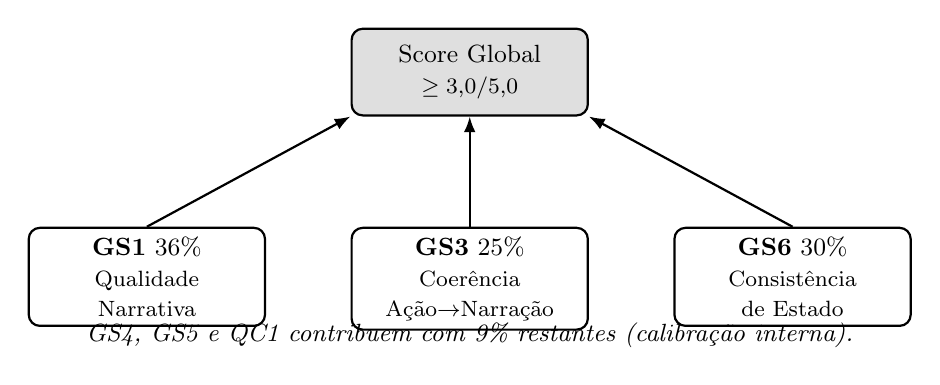
\begin{tikzpicture}[
  every node/.style={font=\small, align=center},
  box/.style={rectangle, rounded corners, draw=black, thick,
              minimum width=3.0cm, minimum height=1.1cm},
  top/.style={box, fill=gray!25},
  arr/.style={-{Latex[length=2mm]}, thick}
]
\node[top] (sg) {Score Global\\\footnotesize $\geq 3{,}0/5{,}0$};
\node[box, below=1.4cm of sg, xshift=-4.1cm] (gs1) {\textbf{GS1} 36\%\\\footnotesize Qualidade\\\footnotesize Narrativa};
\node[box, below=1.4cm of sg]                 (gs3) {\textbf{GS3} 25\%\\\footnotesize Coerência\\\footnotesize Ação$\to$Narração};
\node[box, below=1.4cm of sg, xshift=4.1cm]  (gs6) {\textbf{GS6} 30\%\\\footnotesize Consistência\\\footnotesize de Estado};
\draw[arr] (gs1.north) -- (sg.south west);
\draw[arr] (gs3.north) -- (sg.south);
\draw[arr] (gs6.north) -- (sg.south east);
\node[below=2.5cm of sg, font=\itshape\small] {GS4, GS5 e QC1 contribuem com 9\% restantes (calibração interna).};
\end{tikzpicture}
\caption{Estrutura ponderada das métricas do \texttt{rpg\_judge.py}. GS1+GS3+GS6 perfazem 91\% do score global, refletindo o foco em qualidade do GM LLM; as demais métricas medem calibração do sistema de avaliação interno.}
\label{fig:metricas}
\end{figure}

\subsection{LLM-as-a-Judge}

O modelo avaliador (\textit{judge}) recebe como entrada trechos da sessão (a ação do jogador e a narração gerada pelo MJ), acompanhados de instruções específicas para atribuição de notas em escala Likert (1--5). Cada \textit{prompt} de avaliação é isolado por métrica, evitando que o contexto de uma avaliação influencie outra.

O mesmo \textit{backend} LLM configurado em \texttt{llm\_config.py} pode ser utilizado tanto para geração quanto para avaliação. Embora isso introduza possível circularidade (o modelo tende a avaliar favoravelmente o que ele próprio geraria), essa abordagem é metodologicamente válida conforme Yu et al. \cite{yu:2025}, desde que documentada. Para mitigar o viés, recomenda-se usar modelos diferentes para geração e julgamento nas sessões de avaliação formal. O \texttt{rpg\_judge.py} suporta filtragem por \texttt{session\_id} no \texttt{mundo\_log.csv}, garantindo que apenas eventos da sessão correspondente sejam avaliados nas métricas de mundo aberto (MW1, MW2).

\subsection{Mitigação de Alucinação}

Uma limitação observada em modelos \textit{reasoning} (Gemma~4, DeepSeek-R1, Qwen3) foi a tendência de inventar contexto narrativo não mencionado no \textit{prompt}. A mitigação adotada (instrução explícita ``NUNCA invente personagens, eventos ou contexto não mencionados'' no \texttt{SYSTEM\_PROMPT\_NARRACAO}) reduziu os casos, mas não os eliminou completamente em modelos com temperatura $> 0{,}7$. Modelos \textit{reasoning} também produzem blocos internos \texttt{<think>...</think>} antes de responder. O sistema filtra esses blocos via expressão regular após acumular todo o texto do \textit{stream}, evitando que \textit{tokens} de raciocínio interno apareçam na narração exibida ao jogador.

\subsection{Saídas do Protocolo}

O protocolo produz três artefatos de avaliação:

\begin{itemize}[leftmargin=2.4em]
  \item \textit{scores} por métrica, em escala Likert 1--5;
  \item \textit{score} global agregado, ponderado segundo a Tabela~\ref{tab:metricas};
  \item traços qualitativos de avaliação (justificativas textuais por métrica e por turno).
\end{itemize}

Esses artefatos viabilizam tanto a comparação quantitativa entre modelos quanto a análise qualitativa de modos de falha, conforme detalhado na Seção~\ref{sec:resultados}.

Para fins de referência interna, denominamos o processo de \textit{Structured Interaction Evaluation Pipeline} (SIEP). O desenho assegura que o protocolo capture qualidade local da interação (via GS1 e GS3) e consistência de longo prazo (via GS6), em conformidade com os requisitos R1 (multi-turno) e R2 (consciência de estado). A próxima seção detalha a arquitetura do sistema que implementa o protocolo proposto.

% ─────────────────────────────────────────────────────────────────────────────
\section{Arquitetura do Sistema}
\label{sec:arquitetura}

O protocolo descrito na Seção~\ref{sec:protocolo} é materializado em um \textit{pipeline} modular que processa logs de jogo e produz métricas de avaliação. A arquitetura separa coleta de dados, processamento e avaliação, viabilizando reprodutibilidade e extensibilidade.

\subsection{Visão Geral}

O sistema opera sobre logs estruturados de sessões de RPG, em que cada interação é registrada como uma sequência de eventos. A arquitetura é composta por cinco componentes principais:

\begin{enumerate}[leftmargin=2.4em]
  \item \textbf{Módulo de \textit{Logging}}: registra cada interação em CSV unificado;
  \item \textbf{Módulo de \textit{Parsing} e Filtragem}: normaliza eventos e descarta dados não essenciais;
  \item \textbf{Módulo de Seleção de Segmentos}: isola trechos relevantes (pares ação\,/\,resposta, sequências multi-turno, interações dependentes de estado);
  \item \textbf{Módulo de Avaliação (LLM-as-a-Judge)}: aplica os \textit{prompts} de avaliação por métrica;
  \item \textbf{Módulo de Agregação}: combina notas individuais em \textit{score} global ponderado.
\end{enumerate}

Em paralelo aos cinco componentes do \textit{pipeline} de avaliação, o sistema de jogo é organizado em três camadas funcionais: (1) \textbf{Interface}: questionário narrativo inicial com avaliação LLM e menu de modos; (2) \textbf{Jogo}: motor de combate, mundo aberto e narrativa de NPCs; (3) \textbf{Persistência}: log unificado em CSV, SQLite por coordenada e JSON de estado.

\subsection{Pipeline de Processamento}

O fluxo de avaliação segue cinco etapas sequenciais:

\textbf{Etapa 1 -- Coleta de Logs.} As sessões de jogo são gravadas como logs estruturados em CSV. Cada entrada contém: entrada do jogador, resposta do sistema, tipo de interação (\texttt{avaliacao}, \texttt{narracao\_jogador}, \texttt{narracao\_inimigo}, \texttt{questionario\_p1-5}, \texttt{mundo\_*}) e metadados (\textit{timestamps}, tokens consumidos, tempo de resposta). A partir de Abril de 2026, os campos de entrada e resposta são registrados sem truncamento (até 2000 caracteres), garantindo que narrações completas estejam disponíveis para avaliação.

\textbf{Etapa 2 -- \textit{Parsing} de Eventos.} Os logs são analisados para identificar eventos relevantes. Dados não essenciais são filtrados, e os eventos remanescentes são estruturados em unidades analisáveis.

\textbf{Etapa 3 -- Seleção de Segmentos.} A partir dos eventos analisados, o sistema seleciona trechos adequados à avaliação: pares ação--resposta, sequências multi-turno e interações dependentes de estado. Essa etapa garante que a avaliação se concentre em porções significativas da interação.

\textbf{Etapa 4 -- Avaliação por LLM.} Os segmentos selecionados são enviados ao modelo avaliador, que recebe o segmento de interação, as instruções de avaliação e os critérios de pontuação. O modelo atribui notas para cada métrica segundo as diretrizes fornecidas.

\textbf{Etapa 5 -- Agregação de Métricas.} As notas individuais são combinadas usando os pesos da Tabela~\ref{tab:metricas} para computar médias por métrica e o \textit{score} global, viabilizando comparação entre sessões e modelos.

A Figura~\ref{fig:pipeline} resume o fluxo de dados das cinco etapas: cada \textit{stage} é desacoplado, recebe entrada estruturada e produz saída persistida, possibilitando inspeção, cache e re-execução parcial.

\begin{figure}[ht]
\centering
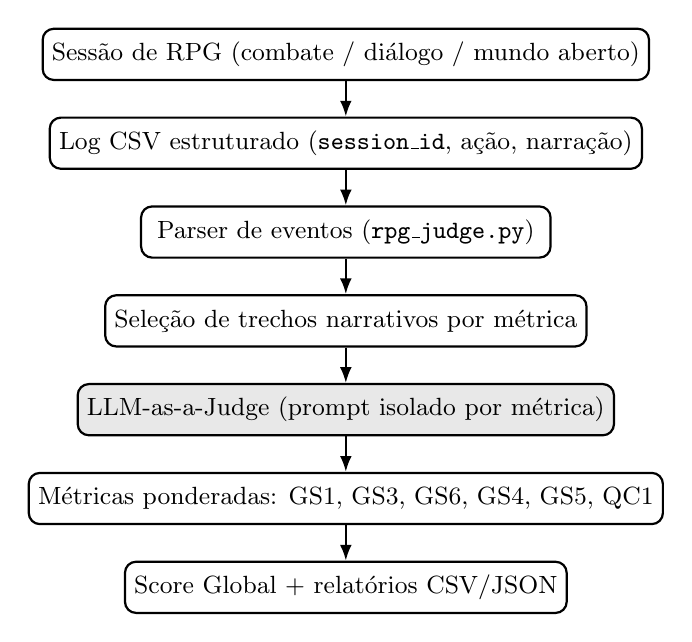
\begin{tikzpicture}[
  node distance=0.45cm,
  every node/.style={
    rectangle, rounded corners, draw=black, thick,
    minimum width=5.2cm, minimum height=0.65cm,
    align=center, font=\small
  },
  judge/.style={fill=gray!18},
  arr/.style={-{Latex[length=2mm]}, thick}
]
\node (a) {Sessão de RPG (combate / diálogo / mundo aberto)};
\node (b) [below=of a] {Log CSV estruturado (\texttt{session\_id}, ação, narração)};
\node (c) [below=of b] {Parser de eventos (\texttt{rpg\_judge.py})};
\node (d) [below=of c] {Seleção de trechos narrativos por métrica};
\node (e) [below=of d, judge] {LLM-as-a-Judge (prompt isolado por métrica)};
\node (f) [below=of e] {Métricas ponderadas: GS1, GS3, GS6, GS4, GS5, QC1};
\node (g) [below=of f] {Score Global + relatórios CSV/JSON};
\foreach \x/\y in {a/b, b/c, c/d, d/e, e/f, f/g} \draw[arr] (\x) -- (\y);
\end{tikzpicture}
\caption{Estrutura do \textit{Structured Interaction Evaluation Pipeline} (SIEP). Logs estruturados são processados em cinco etapas desacopladas e avaliados por um LLM-judge segundo métricas narrativas e de consistência de estado, produzindo um relatório reprodutível independente de avaliação humana.}
\label{fig:pipeline}
\end{figure}

\subsection{Cenário A: Combate}

O Cenário A implementa um \textit{pipeline} de 16 etapas por turno: HUD com arte ASCII por subtipo de inimigo, avaliação LLM de criatividade (0--1) e eficiência (0--2), cálculo de dano, narração em \textit{streaming}, \textit{status effects} (sangramento, veneno, paralisia), progressão de maestria de arma e registro no \texttt{session\_log}. Inclui ainda detecção de ação defensiva que diferencia ações puras (``esquiva'', ``bloqueio'') de ações mistas (``preparo minha esquiva e contra-ataco''); estas últimas são tratadas como ataque normal com componente defensivo, evitando que o jogador burle o sistema de avaliação.

\subsection{Cenário B: Diálogo e Memória de Longo Prazo}

O Cenário B foi originalmente concebido para investigar memória de longo prazo em diálogos investigativos com NPCs; suas funcionalidades foram distribuídas organicamente entre os Cenários A (diálogo após cada quinta batalha, com menu de ações: conversar, descansar, treinar, troca de item, revelação de segredo condicionada a amizade $\geq 60$) e C (comando \texttt{falar~<nome>} no acampamento), ambos chamando o mesmo motor \texttt{NPC.falar()}. A memória de longo prazo é implementada em três camadas: histórico de diálogo por NPC (SQLite, \texttt{memoria\_npc.py}), estado da jornada em JSON (\texttt{jornada.py}) e fatos por coordenada (SQLite do mundo aberto). Ela é re-injetada no \textit{prompt} ao retomar a sessão via \texttt{memoria\_npc.contexto\_para\_llm()}, dimensão coberta pelas métricas GS3 e GS6 do \texttt{rpg\_judge.py} sem demandar um quarto cenário separado.

\subsection{Cenário C: Mundo Aberto}

O Cenário C implementa exploração livre em malha de coordenadas $(x,y,z)$. O bioma é determinado pela distância euclidiana à origem: floresta ($d<2$), planície ($d<5$), deserto/pântano ($d<9$), ruínas ($d>9$), caverna ($z<-2$) e montanha ($z>3$). A Tabela~\ref{tab:modificacoes} lista os tipos de modificação ambiental detectados.

\begin{table}[ht]
\centering
\caption{Modificações ambientais persistentes por coordenada no Cenário C}
\label{tab:modificacoes}
\begin{tabular}{ll}
\toprule
\textbf{Tipo} & \textbf{Palavras-chave detectadas} \\
\midrule
Fogo       & bola de fogo, incêndio, chamas \\
Corte      & corto a árvore, machado, derruba \\
Magia      & conjuro, lanço, raio arcano \\
Escavação  & cavo, escavar, picareta \\
Construção & construo, ergo, barricada \\
Gelo       & congelo, nevar, freeze \\
Explosão   & explodo, blast \\
Água       & inundo, flood \\
\bottomrule
\end{tabular}
\end{table}

Cada local visitado é persistido em SQLite com nome gerado proceduralmente, descrição LLM e histórico de modificações. Ao revisitar um local, o sistema exibe as modificações anteriores no contexto enviado à LLM, mantendo consistência narrativa sem depender de memória interna do modelo. O \texttt{mundo\_log.csv} registra todos os eventos com campo \texttt{session\_id}, permitindo que o \texttt{rpg\_judge} avalie apenas os eventos da sessão correspondente mesmo quando múltiplas sessões compartilham o mesmo arquivo.

\subsection{Integração de Modelos}

A arquitetura suporta múltiplos \textit{backends} de LLM por meio de uma interface unificada (\texttt{llm\_backend.py}), satisfazendo o requisito R4 (operação agnóstica de modelo). Três \textit{backends} são suportados: Ollama (local), LM Studio 0.4.11 (servidor local com API nativa \texttt{/api/v1/chat}) e APIs remotas opcionais (Groq). O \textit{backend} e o modelo são lidos do arquivo \texttt{llm\_config.py} em tempo de execução a cada chamada, sem \textit{cache}, permitindo troca de modelo sem reinicialização. Esse desenho garante que o protocolo de avaliação seja independente de implementações específicas de modelo.

\subsection{Considerações de Reprodutibilidade}

Para assegurar reprodutibilidade (R3), o sistema adota: \textit{prompts} de avaliação fixos e versionados; configuração determinística sempre que possível (temperatura, \textit{seed}, \textit{top-p}); e \textit{logging} explícito dos parâmetros do modelo em cada chamada. Essas medidas permitem que experimentos sejam replicados em ambientes distintos.

Esta arquitetura viabiliza o \textit{pipeline} de avaliação utilizado nos experimentos descritos na Seção~\ref{sec:resultados}, conectando o protocolo conceitual da Seção~\ref{sec:protocolo} à evidência empírica coletada nas 10 sessões instrumentadas.

% ─────────────────────────────────────────────────────────────────────────────
\section{Implementação}

O sistema foi implementado em Python, com o módulo \texttt{rpg\_judge.py} responsável pela avaliação automática. O módulo aceita como entrada um arquivo CSV de sessão isolada ou um diretório completo (processamento em lote), produzindo dois artefatos por execução: um CSV com uma linha por sessão (\texttt{rpg\_judge\_resultados.csv}) e um JSON com estatísticas agregadas por modelo (\texttt{rpg\_judge\_agregado.json}).

\section{Resultados}
\label{sec:resultados}

A Tabela~\ref{tab:resultados} resume os resultados da avaliação preliminar. Os experimentos foram conduzidos sobre uma sessão de referência (69 entradas, 34 narrações, 5 perguntas do questionário) e sessões adicionais com modelos distintos, e apresentam os scores médios obtidos pelas três métricas dominantes e o score global agregado. Para interpretação da escala Likert (1--5): \textbf{scores próximos de 4 indicam desempenho narrativo consistente}, enquanto \textbf{valores abaixo de 3 revelam inconsistências frequentes} (contradições entre turnos, ações narradas incorretamente, ou narração genérica). O limiar de aprovação $\geq 3{,}0$ adotado em RPGBench \cite{yu:2025} marca o piso de utilidade do GM LLM.

\begin{table}[ht]
\centering
\caption{Resultados experimentais por modelo (escala Likert 1--5). $n$ = sessões avaliadas; \textbf{negrito} = melhor por coluna.}
\label{tab:resultados}
\small
\begin{tabular}{lccccc}
\toprule
\textbf{Modelo} & $n$ & \textbf{GS1} & \textbf{GS3} & \textbf{GS6} & \textbf{Global} \\
\midrule
\texttt{qwen2.5:7b-instruct}                           & 1 & \textbf{4{,}79} & \textbf{5{,}00} & 2{,}94          & \textbf{3{,}87} \\
\texttt{gemma4:e2b}~$^{\dagger}$ \cite{deepmind:gemma4:2026} & 1 & 4{,}54          & 4{,}84          & \textbf{2{,}97} & 3{,}70          \\
\texttt{qwen2.5:1.5b}                                  & 7 & 3{,}21          & 4{,}88          & 2{,}21          & 3{,}14          \\
\texttt{qwen2.5:0.5b}                                  & 1 & 3{,}34          & 3{,}52          & 2{,}04          & 3{,}07          \\
\bottomrule
\end{tabular}
\\[2pt]
{\footnotesize $^{\dagger}$ Avaliação obtida após adaptação do parser de saída do \texttt{rpg\_judge.py} para \textit{reasoning models} (\textit{strip} de blocos \texttt{<think>} e busca pelo último JSON balanceado), com taxa de sucesso de parse de 100\% (196/196 chamadas). Antes da adaptação, o mesmo modelo registrava Global $\approx 1{,}9$ devido a falhas de extração: resultado de engenharia de integração, não de capacidade do modelo.}
\end{table}

\textbf{O \texttt{qwen2.5:7b-instruct} e o \texttt{gemma4:e2b} se destacam como os dois únicos modelos a ultrapassarem o limiar de aprovação ($\geq 3{,}0$) em todas as métricas dominantes, com perfis surpreendentemente próximos: 7B-instruct vence em GS1/GS3, e \texttt{gemma4:e2b} (effective 2B) vence em GS6, evidência direta de que arquitetura e regime de treino podem compensar diferença de parâmetros para consistência de estado.} As variantes menores da família Qwen2.5 (1.5B e 0.5B) ficam pouco acima do limiar; \texttt{qwen2.5:1.5b} apresentou alta variância entre sessões (Global $\in [1{,}95;~3{,}72]$, $\sigma=0{,}81$, $n=7$), indicando sensibilidade ao histórico injetado e ao estilo do jogador. Conforme nota da Tabela~\ref{tab:resultados}, o salto de \texttt{gemma4:e2b} de $\approx 1{,}9$ para $3{,}70$ após adaptação do parser para \textit{reasoning models} ilustra que engenharia de integração pode ser o limite efetivo, não a capacidade do modelo. \textbf{GS6 (consistência de estado) permanece como o gargalo principal:} mesmo o melhor modelo fica em $2{,}97$, no piso do limiar, e a coerência de longo prazo continua sendo o limite duro de modelos de pesos abertos sub-10B. GS3 satura próximo de $5{,}00$ nos modelos $\geq 1{,}5$B, indicando que ações simples são fielmente narradas. Embora limitados em escala ($n=10$ sessões, quatro modelos, três cenários), estes resultados são suficientes para demonstrar a \textit{capacidade discriminativa} do protocolo proposto: as métricas separam modelos com perfis distintos de forma reprodutível e expõem o gargalo de consistência como direção prioritária para futuras versões.

\textbf{Modos de Falha Observados.} A análise qualitativa revelou cinco padrões sistemáticos, mais frequentes em modelos abaixo de 7B:

\begin{enumerate}[label=(\roman*),leftmargin=2.4em,itemsep=2pt]
  \item \textbf{Vazamento de variáveis internas}: \texttt{qwen2.5:0.5b} adicionou ao JSON de saída campo não solicitado (\texttt{"necessita de contexto envolvente"});
  \item \textbf{Alucinação propagada via histórico contaminado}: nome incorreto do jogador (\textit{``Silvano''}) propagou-se entre sessões e modelos (\texttt{qwen2.5:1.5b} e \texttt{gemma4:e2b});
  \item \textbf{Quebra de persona com meta-desculpas}: \texttt{qwen2.5:1.5b} respondeu como assistente técnico (\textit{``Peço desculpas pela confusão anterior...''}) em vez de manter o NPC;
  \item \textbf{Vazamento de prefixos do log}: \texttt{gemma4:e2b} reproduziu literalmente rótulos estruturais (\texttt{Yara:}, \texttt{Fe:});
  \item \textbf{Admissão de limitação técnica}: modelo justificou ausência de informação como \textit{``não tenho a capacidade''}, em vez de criar barreira narrativa.
\end{enumerate}

Quanto ao ritmo, falhas ocorreram já no turno~0 quando o histórico injetado continha erros de testes anteriores, e entre os turnos~1 e~4 em diálogos com NPCs, por acúmulo de contexto excedendo a janela de atenção dos modelos pequenos a instruções negativas (\textit{``não saia da persona''}).

\textbf{Limitações.} \textit{LLM-as-a-judge não é \textit{ground truth}}: fornece estimativa correlacionada (não equivalente) ao julgamento humano, com erros sistemáticos. Quatro limitações principais:

\begin{enumerate}[label=(\arabic*),leftmargin=2.4em,itemsep=2pt]
  \item \textit{viés do avaliador}: o judge favorece estilos próximos ao seu padrão de geração;
  \item \textit{dependência de prompts}: pequenas variações no \textit{prompt} alteram notas significativamente;
  \item \textit{circularidade}: mesmo modelo gerando e julgando pode superestimar qualidade; mitigada usando \texttt{qwen2.5:7b-instruct} como judge e demais como geradores;
  \item \textit{ausência de avaliação humana formal das narrativas}: as 3 sessões foram conduzidas por jogadores reais (variância de estilo), mas nenhuma escala subjetiva de imersão foi coletada; o judge correlaciona com julgamento humano em tarefas abertas \cite{zheng:2023} sem substituir percepção subjetiva. Validação por \textit{survey} é direção de trabalho futuro.
\end{enumerate}

% ─────────────────────────────────────────────────────────────────────────────
\section{Conclusão}

Este trabalho apresentou um protocolo reprodutível de avaliação para Mestres de Jogo baseados em LLM, materializado no módulo \texttt{rpg\_judge.py} e operando sobre um sistema de GM autônomo com três cenários (combate, diálogo e mundo aberto) executando em LLMs locais. A arquitetura de persistência em três camadas (SQLite, JSON, CSV) mostrou-se eficaz para consistência narrativa, e as métricas implementadas são comparáveis às propostas em RPGBench \cite{yu:2025}. \textbf{O protocolo proposto não se restringe a RPGs}: a estrutura de logs estruturados, métricas ponderadas e LLM-as-a-judge é aplicável a outros sistemas interativos baseados em LLM, como assistentes narrativos, agentes conversacionais de longa duração e simulações educacionais de \textit{role-play}, ampliando seu potencial de impacto além do escopo deste trabalho.

Como trabalho futuro, pretende-se: (1) validação com avaliadores humanos para correlacionar as métricas automáticas com percepção subjetiva de qualidade; (2) uso de múltiplos modelos \textit{judge} para reduzir o viés de circularidade e aumentar a robustez das avaliações; (3) refinamento das métricas narrativas com análise de diversidade lexical (TTR, MTLD) conforme Reviriego et al. \cite{reviriego:2024}; (4) integração de banco vetorial FAISS para memória semântica de longo prazo; (5) expansão do Cenário C com encontros de diálogo no mundo aberto.

\textbf{Agradecimentos.} [OMITIDO PARA REVISÃO ANÔNIMA]

\bibliographystyle{sbc}
\bibliography{Referencias/referencias}

\end{document}
